%% The lines that are not written within % .. % are not to be tampered with!!

\documentclass[twoside]{article}
\setlength{\oddsidemargin}{0.25 in}
\setlength{\evensidemargin}{-0.25 in}
\setlength{\topmargin}{-0.6 in}
\setlength{\textwidth}{6.5 in}
\setlength{\textheight}{8.5 in}
\setlength{\headsep}{0.75 in}
\setlength{\parindent}{0 in}
\setlength{\parskip}{0.1 in}

%
% ADD PACKAGES here:
\usepackage{amssymb}
\usepackage{multirow}

\usepackage[most]{tcolorbox} % 引入 tcolorbox 宏包
\usepackage{amsthm}
\usepackage{xcolor}
\usepackage{amsmath,amsfonts,graphicx}
\usepackage{etoolbox} % 提供 \BeforeBeginEnvironment 和 \AfterEndEnvironment
\usepackage{graphicx}
\usepackage{tikz}
\tikzset{
    level distance=2cm,
    sibling distance=2.5cm
}

\newtheoremstyle{definitionstyle}
  {3pt}   % 上方间距
  {3pt}   % 下方间距
  {\normalfont} % 字体
  {}      % 缩进
  {\bfseries\color{blue}} % 标题字体
  {.}     % 标题后标点
  {0.5em} % 标题后间距
  {}      % 标题格式
\theoremstyle{definitionstyle}
\newtheorem*{definition}{Definition}
\newtheorem*{theorem}{Theorem}  
\BeforeBeginEnvironment{definition}{%
  \begin{tcolorbox}[
    colback=white,
    colframe=black,
    boxrule=0.6pt, % 边框粗细
    arc=0pt,       % 直角
    top=4pt,       % 上内边距
    bottom=4pt,    % 下内边距
    left=4pt,      % 左内边距
    right=4pt,     % 右内边距
    breakable,     % 允许跨页
  ]%
}
\AfterEndEnvironment{definition}{\end{tcolorbox}}

\BeforeBeginEnvironment{theorem}{
  \begin{tcolorbox}[
    colback=white,
    colframe=black,
    boxrule=0.6pt, % 边框粗细
    arc=0pt,       % 直角
    top=4pt,       % 上内边距
    bottom=4pt,    % 下内边距
    left=4pt,      % 左内边距
    right=4pt,     % 右内边距
    breakable,     % 允许跨页
  ]%
}
\AfterEndEnvironment{theorem}{\end{tcolorbox}}

\newcounter{lecnum}
\renewcommand{\thepage}{\thelecnum-\arabic{page}}
\renewcommand{\thesection}{\thelecnum.\arabic{section}}
\renewcommand{\theequation}{\thelecnum.\arabic{equation}}
\renewcommand{\thefigure}{\thelecnum.\arabic{figure}}
\renewcommand{\thetable}{\thelecnum.\arabic{table}}


\newcommand{\lecture}[4]{
   \pagestyle{myheadings}
   \thispagestyle{plain}
   \newpage
   \setcounter{lecnum}{#1}
   \setcounter{page}{1}
   \noindent
   \begin{center}
   \framebox{
      \vbox{\vspace{2mm}
    \hbox to 6.28in { {\bf MATH4321} }
       \vspace{4mm}
       \hbox to 6.28in { {\Large \hfill Lecture #1: #2  \hfill} }
       \vspace{2mm}
      \vspace{2mm}}
   }
   \end{center}
   \markboth{Lecture #1: #2}{Lecture #1: #2}
}



\renewcommand{\cite}[1]{[#1]}
\def\beginrefs{\begin{list}%
        {[\arabic{equation}]}{\usecounter{equation}
         \setlength{\leftmargin}{2.0truecm}\setlength{\labelsep}{0.4truecm}%
         \setlength{\labelwidth}{1.6truecm}}}
\def\endrefs{\end{list}}
\def\bibentry#1{\item[\hbox{[#1]}]}

%Use this command for a figure; it puts a figure in wherever you want it.
%usage: \fig{NUMBER}{SPACE-IN-INCHES}{CAPTION}
%This is for your help while typing the notes
\newcommand{\fig}[3]{
			\vspace{#2}
			\begin{center}
			Figure \thelecnum.#1:~#3
			\end{center}
	}

\newcommand\E{\mathbb{E}}
\newcommand{\PI}{$P_{i}$}
\newcommand{\KIA}{$K_{i}(A)$}
\newcommand{\FIW}{$F_{i}(\omega)$}
\newcommand{\OS}{$\omega ^{*}$}
\begin{document}
\lecture{2}{Dynamic games: Games in extensive form}{XIE}{}


\section{Dynamic games: Perfect information}
players make their decision sequentially (instead of simultaneously).\\
unique feature:  some players can acquire additional information about the games\\
dynamic games: set of players; order of moves; information set; strategic set; payoffs\\
\begin{definition}[Information set]
  We let $N_i$ be the set of nodes that player $i$ needs to make her next decision at a particular stage. The \textit{information set} of a player $i$ at node $x$, denoted by $h_i(x)$, is an element of the partition of $N_i$ that describe the player $i$'s knowledge about her position at that stage. 
\end{definition}
The information set contains all the possibilities of the players. 
%
%
%
\begin{definition}[Perfect information and imperfect information]
  A game of extensive form is said to be of \textit{perfect information} if every information set consists of a single element. 
On the other hand, a games is said to be of \textit{imperfect information} if some information sets consist of two or more elements. 
\end{definition}
We say a games is of perfect information if all players can acquire the full 
information about strategies chosen by the players in earlier rounds and the events happened in the past.
%
%
%
\begin{definition}[Pure strategy in dynamic games]
  We let $I={h_i(x): x\in N_i}$ be a collection of possible information sets of player $i$ and $S_i$ be the strategic set of player $i$. A player $i$'s pure strategy is defined as a function $s_i:I\rightarrow S_i$ which assigns a single strategy in $S_i$ to every information set $h_i(\cdot)\in I$. 
\end{definition}
Remark: If $h_i(x) = h_i(x')$, we must have $s_i(h_i(x)) = s_i(h_i(x'))$
%
%
%
\begin{definition}[Nash equilibrium for pure strategy]
  A strategic profile $s^*=(s_1^*,s_2^*,...,s_n^*)$ constitutes pure strategy Nash 
equilibrium if and only if for any player $i$
$$V_i(s_i^*;s_{-i}^*)=\max_{s_i\in S_i}V_i(s_i;s_{-i}^*) $$
or equivalently, 
$$V_i(s_i^*;s_{-i}^*) \geq V_i(s_i;s_{-i}^*), \text{for any }s_i\in S_i \dots(*) $$
\end{definition}
%
%
%
%example 8
Example 8(voting game)
Tony and Sunny will have a short-trip in the coming summer. They choose to visit one of the following places: Singapore (S), Japan (J) or Taiwan (T). It is known that:
\begin{itemize}
    \item Tony's preference is given by $\underbrace{S}_{1^{st} \text{ choice}} > \underbrace{J}_{2^{nd} \text{ choice}} > \underbrace{T}_{3^{rd} \text{ choice}}$.
    \item Sunny's preference is given by $\underbrace{J}_{1^{st} \text{ choice}} > \underbrace{T}_{2^{nd} \text{ choice}} > \underbrace{S}_{3^{rd} \text{ choice}}$.
\end{itemize}

Two people must choose among these 3 choices. The game is as follows: Sunny first decides and rules out one of the three choices. Then Tony chooses to rule out one of the remaining two choices. Depending on the final outcome $F$, the player's payoff is assumed to be:
\[
V_i(1^{st} \text{ choice}) = 3, \quad V_i(2^{nd} \text{ choice}) = 2, \quad V_i(3^{rd} \text{ choice}) = 1.
\]
Determine all possible pure strategy Nash equilibrium for this game.

\vspace{0.3cm}
\textbf{Solution}

We first express the game into game tree form. Since Tony will rule out one of the choices from the remaining two, he should know the choice that is eliminated by Sunny (Leader). Thus the game is of perfect information. Given the payoffs profile, the game tree can be expressed as:

\begin{center}
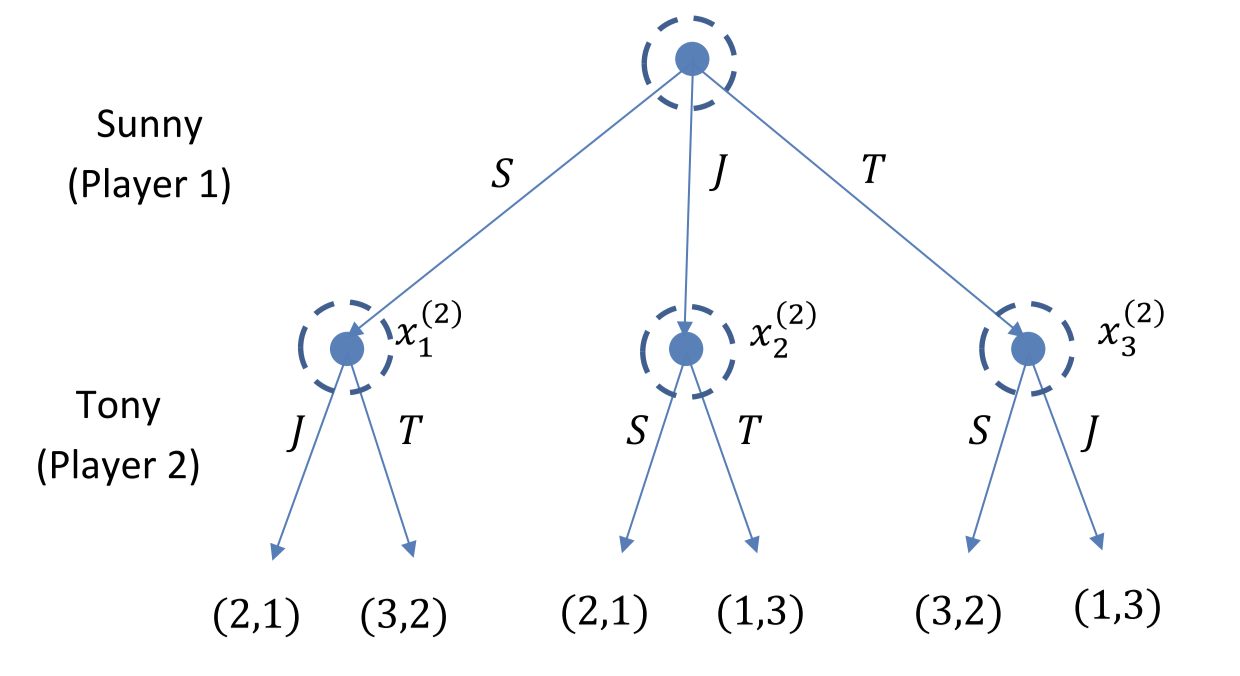
\includegraphics[width=0.8\textwidth]{example 8 (voting game)_L2.png}
\end{center}

The pure strategies of these two players can be expressed as:
\[
s_1 = s_1(x_1^{(1)}), \quad s_2 = \big(s_2(x_1^{(2)}), s_2(x_2^{(2)}), s_2(x_3^{(2)})\big),
\]
where $s_1(x_1^{(1)}) \in \{S, J, T\}$, $s_2(x_1^{(2)}) \in \{J, T\}$, $s_2(x_2^{(2)}) \in \{S, T\}$ and $s_2(x_3^{(2)}) \in \{S, J\}$.

The corresponding matrix form of this game is given by:

\vspace{0.3cm}
\begin{center}
\begin{tabular}{|c|c|c|c|c|c|c|c|c|}
\hline
& \multicolumn{8}{c|}{Tony (Player 2)} \\
\cline{2-9}
& $(J,S,S)$ & $(J,S,J)$ & $(J,T,S)$ & $(J,T,J)$ & $(T,S,S)$ & $(T,S,J)$ & $(T,T,S)$ & $(T,T,J)$ \\
\hline
$S$ & (2,1) & (2,1) & (2,1) & (2,1) & (3,2) & (3,2) & (3,2) & (3,2) \\
\hline
$J$ & (2,1) & (2,1) & (1,3) & (1,3) & (2,1) & (2,1) & (1,3) & (1,3) \\
\hline
$T$ & (3,2) & (1,3) & (3,2) & (1,3) & (3,2) & (1,3) & (3,2) & (1,3) \\
\hline
\end{tabular}
\end{center}

\vspace{0.3cm}
For each player $i$, we determine his best response $s_i^*$ to every opponent's (player $j$, $j \neq i$) strategy. The best responses of the players are summarized in the matrix below (with upper bar):

\vspace{0.3cm}
\begin{center}
\begin{tabular}{|c|c|c|c|c|c|c|c|c|}
\hline
& \multicolumn{8}{c|}{Tony (Player 2)} \\
\cline{2-9}
& $(J,S,S)$ & $(J,S,J)$ & $(J,T,S)$ & $(J,T,J)$ & $(T,S,S)$ & $(T,S,J)$ & $(T,T,S)$ & $(T,T,J)$ \\
\hline
$S$ & (2,1) & (\underline{2},1) & (2,1) & (\underline{2},1) & (\underline{3},\underline{2}) & (\underline{3},\underline{2}) & (\underline{3},\underline{2}) & (\underline{3},\underline{2}) \\
\hline
$J$ & (2,1) & (\underline{2},1) & (1,\underline{3}) & (1,\underline{3}) & (2,1) & (2,1) & (1,\underline{3}) & (1,\underline{3}) \\
\hline
$T$ & (\underline{3},2) & (1,\underline{3}) & (\underline{3},2) & (1,\underline{3}) & (\underline{3},2) & (1,\underline{3}) & (\underline{3},2) & (1,\underline{3}) \\
\hline
\end{tabular}
\end{center}

\vspace{0.3cm}
We observe that there are four Nash equilibria in this game: 
\[
s_1^* = (S, (T, S, S)), \quad s_2^* = (S, (T, S, J)), \quad s_3^* = (S, (T, T, S)), \quad s_4^* = (S, (T, T, J)).
\]

Furthermore, these equilibria induces a common outcome: Sunny first rules out the choice "$S$" (Singapore) and Tony rules out the choice "$T$" (Taiwan). So the remaining choice will be "$J$" (Japan).
%
%
%
\begin{definition}[Sequential rationality]
  We let $s_{-i}$ be the strategy chosen by the opponents. We say that a player $i$'s strategy $s_i$ is \textbf{sequentially rational} if and only if $s_i$ is a best response to $s_{-i}$ in any information set $h_i(x)$ of player $i$. That is,
\[
V_i(s_i; s_{-i}) \mid_{h_i(x)} \;=\; \max_{s}\; V_i(s; s_{-i}) \mid_{h_i(x)}.
\]
\end{definition}
%
%
%
\begin{definition}[Sequentially rational Nash equilibrium]
  A pure strategy Nash equilibrium $s^* = (s_1^*, s_2^*, \dots, s_n^*)$ is said to be a \textbf{sequentially rational Nash equilibrium} if and only if $s_i^*$ is sequentially rational (with respect to $s_{-i}^*$) for any player $i$. That is,
\[
V_i(s_i^*; s_{-i}^*) \mid_{h_i(x)} = \max_{s} V_i(s; s_{-i}^*) \mid_{h_i(x)}
\]
for any information set $h_i(x)$.
\end{definition}
%
%
%
\textbf{Backward induction}: example: \\
As an example, we revisit the voting games in Example 8. One can use backward induction and find the Nash equilibrium as follows:

\textbf{Step 1:} We first consider the second stage where Tony makes the last move. Knowing the strategy made by Sunny previously, Tony's decision problem is equivalent to a single-person optimization problem.
\begin{center}
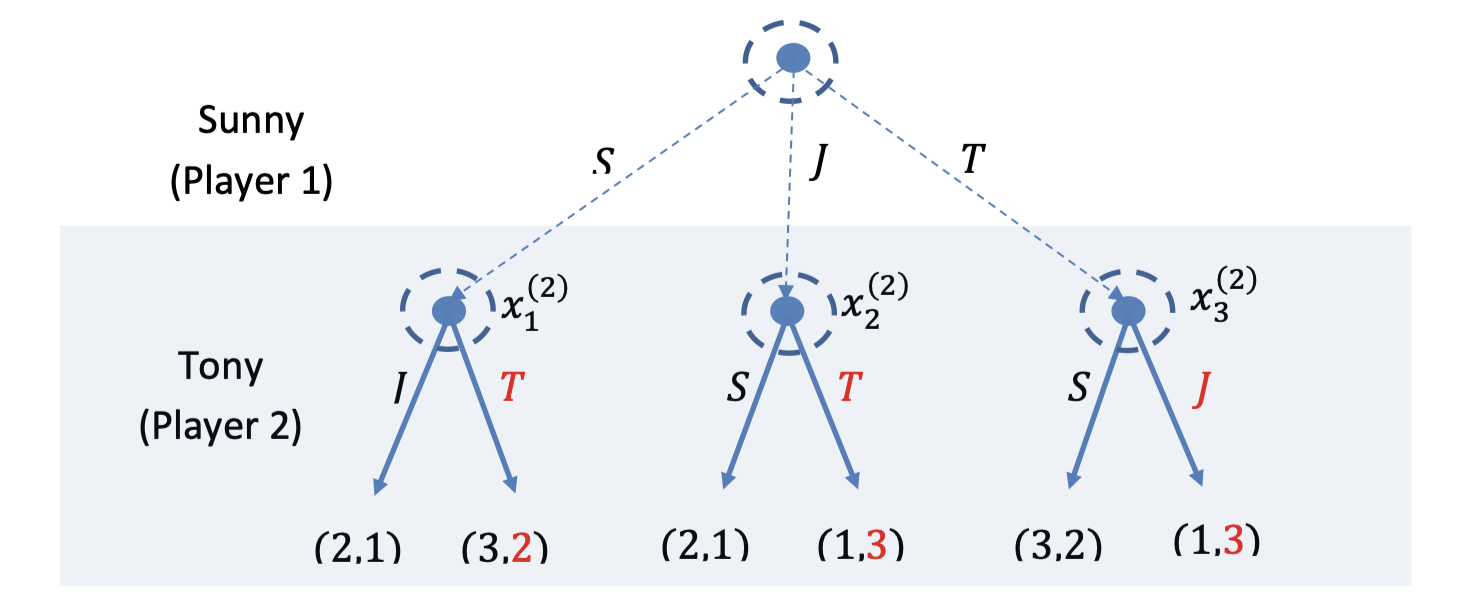
\includegraphics[width=0.8\textwidth]{eg_sequential_logic.png}
\end{center}
From the game tree, we deduce that Tony's optimal strategy is given by
\[
s_2^*(x_1^{(2)}) = T, \quad
s_2^*(x_2^{(2)}) = T, \quad
s_2^*(x_3^{(2)}) = J.
\]

\textbf{Step 2:} We move to first stage and determine Sunny's optimal strategy. Knowing that Tony should make his decision rationally, Sunny can ``forecast'' Tony's strategy under various scenarios. So his optimization problem can now be reduced into a single-person problem again.
\begin{center}
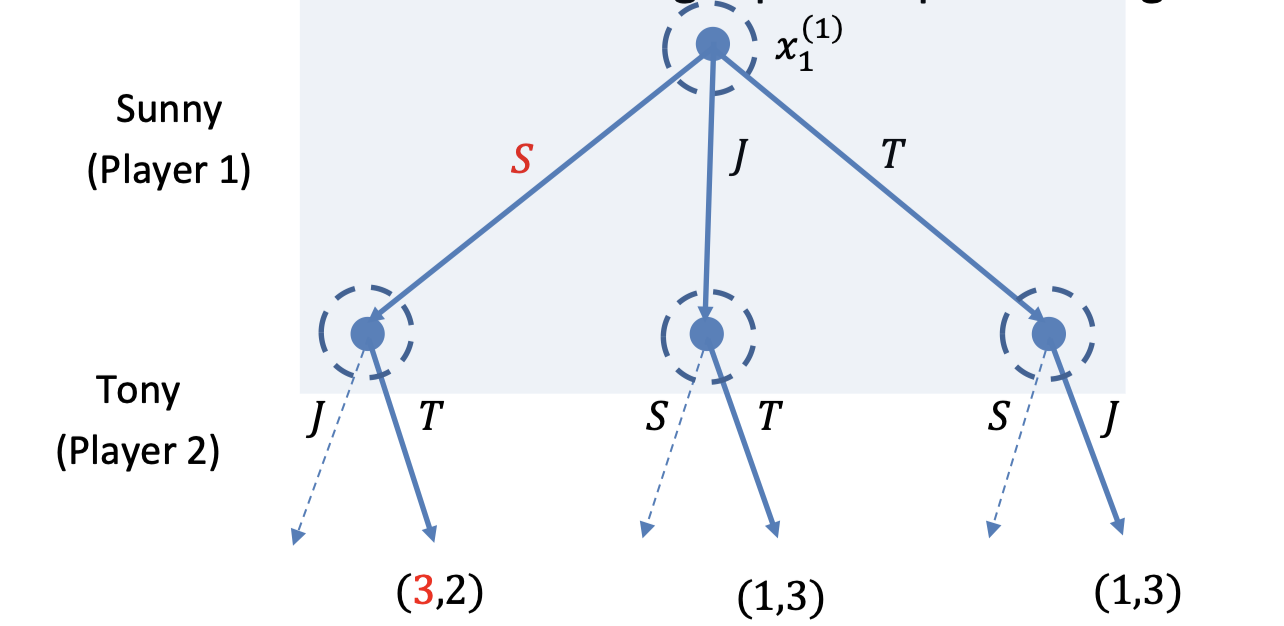
\includegraphics[width=0.8\textwidth]{eg_sequantial_logic2.png}
\end{center}
We deduce from the above tree that Sunny's optimal strategy is
\[
s_1^*(x_1^{(1)}) = S.
\]

Thus, $s^* = (S, (T, T, J))$ is the potential sequentially rational Nash equilibrium.
%
%
%
\begin{theorem}
  For any games of perfect information, the strategic profile $s^*$ (in pure strategy) obtained through backward induction is the sequentially rational Nash equilibrium. Furthermore, such equilibrium always exist for every games of perfect information. 
\end{theorem}
Remark (Uniqueness of solution):\\
The equilibrium is uniquely determined if there do not exist two terminal nodes that yields the same payoffs to any player. \\
%
%
%
%
%
\section{Dynamic games: imperfect information}
\begin{definition}[Subgames]
  We let G be a games in extensive form. We say G' is a proper subgame 
of G if it has the following properties: \\
(1) It has a single initial node; \\
(2) For every node $x \in G' $and any $y\in h(x)$, we must have $y\in G'$. \\
(In other words, the player's optimal strategies in the subgames does not depend on any information outside the subgames.) 
\end{definition}
For imperfect information, notice that since you do not know what decision other players might do, so different 
decisions made by them should be bound to one information set(connected)\\
\newline
%
may not be able to find optimal decision in every stage due to lack of information, thus we consider subgames 
\begin{definition}[Subgame perfect equilibrium]
A strategic profile $s^*=(s_1^*, s_2^*, \dots, s_n^*)$ is said to be a subgame perfect 
equilibrium in a dynamic games G if and only if $s^*$ is Nash equilibrium in every proper subgames G' in G.  
\end{definition}
Remark:\\
1. To solve this NE, we do backward to proper subgames instead of stages.\\
2. For the games of perfect information, the set of subgame perfect equilibrium is same as the set of sequentially rational Nash equilibrium obtained by standard backward induction. \\
3. the method is same as above, find optimal payoff of the lowest subgame, then use the payoff to calculate backward\\

\subsection{Application 1: Multi-stage games and repeated games:} 

the games consists of a finite number of normal-form games $G_1, G_2, G_3, \ldots , G_N$, all are independent static games played sequentially, and result of $G_i$ is known after it is played.\\
\textbf{Total discounted payoff of player i} = $V_i(s_i, s_{-i}) = V_i^{(1)} + DV_i^{(2)}+D^2V_i^{(3)} + \ldots + D^{N-1}V_i^{(N)} = \sum_{j=1}^N D^{j-1}V_i^{(j)}$\\
\textbf{example}: bank income of time deposit\\
\textbf{information set}: For $k = 1,2, \ldots , N$, we let $h_i(k)$ be the information set of player i at k-th
stage in which the games $G_1, G_2, G_3, \ldots , G_{k-1}$ have been played. Then $h_i(k)$ can 
be (informally) described as \\
$h_i^{(k)} = h^{(k)}$ = outcomes of games $G_1, G_2, G_3, \ldots , G_{k-1}$ = $\{s^{(1)}, s^{(2)}, \ldots, s^{(k-1)}\}$,\\
where $\{s^{(j)} = s_1^{(j)}, s_2^{(j)}, \ldots, s_n^{(j)}\}$ denotes the strategy chosen by the 
players in games $G_j$. \\
$s_i^{(k)}$ is a function of her information set at this stage, i.e. $s_i^{(k)} = s_i^{(k)}(h_i^{(k)})$\\
\textbf{solution:} for $G_N$, equilibrium strategy = Nash equilibrium in $G_N$\\
Suppose the equilibrium strategy in games $G_{k+1}, \ldots, G_N$ has been obtained and we consider $G_k$, each player chooses her strategy in game $G_k$ to maximize the total payoffs $V_i^{(k)}+DV_i^{(k+1)}+\ldots + D^{N-k}V_i^{(N)}$ \\
\begin{theorem}
  We let $s^{(j)*} = (s_1, s_2^{(j)}, \ldots, s_n^{(j)})$ be a Nash equilibrium in the subgame $G_j(j = 1,2, \ldots, n)$. The strategic profile $s^* = s^{(1)*}, s^{(2)*}, \ldots, s^{(N)*}$ is the 
subgame perfect equilibrium of the multi-stage games. 
\end{theorem}
(prove by backward)\\
Conditional strategy: subgames are not independent: \\
1. when doing backward, mind that there would be some restrictions\\
2. usually we balance long-term loss and short-term loss with Conditional strategy, instead of reaching equilibrium at every stage\\
3. you can set the condition yourself, as long as it is valid(prove this strategy is a NE in all subgames)\\
\newline
players' behavior in earlier subgames may not necessarily to be Nash equilibrium in that subgames. Conditions are:\\ 
1. There exists two or more Nash equilibria in some subgames at later stage. This condition is necessary so that the players can “force” other players to adopt a particular strategy at earlier stage by offering some “rewards” or “penalty” in later games: Adopt different strategies for different outcomes in earlier games. \\
2. The value of discount factor D. The discount factor affects the players' payoff at later games, this would affect the players' incentives to deviate from the equilibrium strategies at the earlier subgames. \\
\newline
\textbf{example 23:}\\
Two companies (Company 1 and 2) work on two investment projects ($P_1, P_2$) together. Two projects are conducted in different periods: $P_1$ is conducted at period 1 and $P_2$ is conducted at period 2 .

\begin{itemize}
    \item In the first project $P_1$, two companies decide simultaneously the amount of effort (high (H) or low (L)) to be invested in the project. The companies' payoffs in $P_1$ are summarized by the following matrix :
    \[
    \begin{array}{r|c|c|}
    \multicolumn{1}{r}{} & \multicolumn{1}{c}{\text{H}} & \multicolumn{1}{c}{\text{L}} \\ \cline{2-3}
    \text{H} & (5, 5) & (2, 6) \\ \cline{2-3}
    \text{L} & (6, 2) & (3, 3) \\ \cline{2-3}
    \end{array}
    \]
    
    \item In the second project $P_2$, two companies decide whether to put effort (E) in the project \cite{298}. The project is successful only when both companies choose to put effort. The companies' payoffs in $P_2$ are summarized by the following matrix:
    \[
    \begin{array}{r|c|c|}
    \multicolumn{1}{r}{} & \multicolumn{1}{c}{\text{E}} & \multicolumn{1}{c}{\text{N}} \\ \cline{2-3}
    \text{E} & (5, 3) & (-2, 0) \\ \cline{2-3}
    \text{N} & (0, -2) & (0, 0) \\ \cline{2-3}
    \end{array}
    \]
    (\textit{*Note: ``N'' denotes ``no effort''} .)
\end{itemize}

The total payoffs of company $i$ is assumed to be $V_i = V_i^{(1)} + D V_i^{(2)}$, where $V_i^{(1)}$ and $V_i^{(2)}$ are the payoffs received by company $i$ in $P_1$ and $P_2$ respectively . Here, $D \in [0,1]$ denotes the discount factor over 1 period.

If the company conducts the first project $P_1$ only, one can show that $(s_1^*, s_2^*) = (L, L)$ and both companies choose to put small effort in $P_1$. This example examines whether the inclusion of the second project $P_2$ can give companies some incentives to increase their effort in the first project.
Show that when $D$ is sufficiently large, there is a subgame perfect equilibrium in which two companies choose $H$ in $P_1$.

\textbf{Solution}:\\
To obtain the required subgame perfect equilibrium, we apply backward induction and first find all Nash equilibria in the last game (project $P_2$). The best responses of the companies in $P_2$ are marked (with an overline) in the following matrix:
\[
\begin{array}{r|c|c|}
\multicolumn{1}{r}{} & \multicolumn{1}{c}{\text{E}} & \multicolumn{1}{c}{\text{N}} \\ \cline{2-3}
\text{E} & (\overline{5}, \overline{3}) & (-2, 0) \\ \cline{2-3}
\text{N} & (0, -2) & (\overline{0}, \overline{0}) \\ \cline{2-3}
\end{array}
\]
We observe that there are two Nash equilibria [namely, $(E, E)$ and $(N, N)$] in the last game.

Next, we proceed to determine the optimal strategies in the first project $P_1$. In order to ``encourage'' two companies to choose $(H, H)$ in the first game, we take the companies' conditional strategies in $P_2$ to be:
\[
\left( s_1^{(2)*}(h^{(1)}), s_2^{(2)*}(h^{(1)}) \right) = 
\begin{cases} 
(E, E) & \text{if } (s_1^{(1)}, s_2^{(1)}) = (H, H) \\ 
(N, N) & \text{if otherwise} 
\end{cases} \quad \cdots \quad (1)
\]
In other words, each company tries to threaten another company by choosing $N$ (not to put effort in the second project) if anyone cheats and plays $L$ in the first stage.

Given the conditional strategy choice (1), the payoffs of the entire game under various actions in $P_1$ can be expressed by the following matrix form:
\[
\begin{array}{r|c|c|}
\multicolumn{1}{r}{} & \multicolumn{1}{c}{\text{H}} & \multicolumn{1}{c}{\text{L}} \\ \cline{2-3}
\text{H} & (5 + 5D, 5 + 3D) & (2 + 0D, 6 + 0D) \\ \cline{2-3}
\text{L} & (6 + 0D, 2 + 0D) & (3 + 0D, 3 + 0D) \\ \cline{2-3}
\end{array}
\]
which simplifies to:
\[
\begin{array}{r|c|c|}
\multicolumn{1}{r}{} & \multicolumn{1}{c}{\text{H}} & \multicolumn{1}{c}{\text{L}} \\ \cline{2-3}
\text{H} & (5 + 5D, 5 + 3D) & (2, 6) \\ \cline{2-3}
\text{L} & (6, 2) & (3, 3) \\ \cline{2-3}
\end{array}
\]

For $(H,H)$ to be a valid Nash equilibrium in the first stage (thereby sustaining mutual high effort), no player should have an incentive to unilaterally deviate. We check the equilibrium conditions for both companies:\\

\textbf{For Company 1:}\\
If Company 2 plays $H$, Company 1 can get $5 + 5D$ by playing $H$, or get $6$ by deviating to $L$. To ensure Company 1 prefers $H$:
$5 + 5D \ge 6$, thus $D \ge \frac{1}{5}$\\
\textbf{For Company 2:}\\
If Company 1 plays $H$, Company 2 can get $5 + 3D$ by playing $H$, or get $6$ by deviating to $L$. To ensure Company 2 prefers $H$:
$5 + 3D \ge 6$, thus $D \ge \frac{1}{3}$ \\
By combining these bounds, we require:
$D \ge \max\left( \frac{1}{5}, \frac{1}{3} \right) = \frac{1}{3}$\\
\newline
\textbf{Conclusion:}\\
When $D \ge \frac{1}{3}$ (i.e., $D$ is sufficiently large), neither company has an incentive to choose $L$ in $P_1$. Thus, the specified strategic profile forms a valid Subgame Perfect Equilibrium where both companies choose $H$ in $P_1$.\\
\newline
%
%
%
Remark:\\
1. you need to show that normally, it has no incentive to deviate\\
2. if it deviate, then there would be punishment, and all players have incentive to carry on punishment strategy\\
\text{***}\\
define $s_i^{(s,h_i)}$ to be $s_i^{(s,h_i)} = s_i^{(s, h_i)}(h) = 
\begin{cases} 
s & \text{if } h = h_i, \\ 
s_i & \text{if } h \neq h_i. 
\end{cases}$ to represent an one-stage deviation(only deviate at this particular information set $h_i$)
\begin{definition}[One-stage unimprovable]
  A player i's strategy $s_i$ is said to be one-stage unimprovable with respect to the opponents' strategy $s_{-i}$ if there is no information set $h_i$ and 
strategy $s\in S_i$ such that $V_i(s_i^{(s,h_i)}; s_{-i})|_{h_i}>V_i(s_i; s_{-i})|_{h_i}$. In other words, player i cannot get any additional benefit by adopting any one-stage deviation strategy. 
\end{definition}
\begin{theorem}[One-stage deviation principle]
  If a strategy $s_i^*$ is one-stage unimprovable with respect to $s_{-i}^*$ for any player i, then the strategic profile $s^* = (s_1^*, s_2^*, \ldots, s_n^*)$ is the subgame perfect equilibrium in a dynamic games. 
\end{theorem}
%
%
%
\textbf{repeated games}:\\
Repeated games is a kind of multi-stage games in which players play a 
particular game G repeatedly.  There are two types of repeated games: (1) finite repeated games and (2) infinite repeated games. \\
\newline
\textbf{finite repeated games}: Suppose that the games G is played for n times, let $V_i^{(j)}$ be the player i's 
payoff in the j-th round. define total payoff of player i as: $V_i(s_i, s_{-i})=\sum_{j=1}^nD^{j-1}V_i^{(j)}(s_i^{(j)}; s_{-i}^{(j)})$\\
Remark:\\
1. Suppose you have a 10 round game with strategies x, y, z and you want it to choose strategy x, then you need to perform standard NE in the last round, i.e. setting rewards using the last round to ensure that x would be optimal in previous 9 rounds.\\
2. you can play non-equilibrium strategy x in G under SPE if y Pareto dominate z, and x Pareto dominate y, z\\
\newline
\textbf{infinite repeated games}:\\
let $s_i^{(j)} = s_i^{(j)}(h_i^{(j)})$ be player i's strategy at j-th round, $s_i = (s_i^{(1)}, s_i^{(2)}, \ldots)$, payoff of player i: $V_i = V_i(s_i^{(1)}; s_{-i}^{(1)}) + DV_i(s_i^{(2)}; s_{-i}^{(2)})+ D^2V_i(s_i^{(3)};s_{-i}^{(3)}) + \ldots$, assume $V_i^{(j)}$ is bounded\\
\begin{theorem}
  Suppose $a^* = (a_1^*, a_2^*, \ldots, a_n^*)$ is a pure strategy Nash equilibrium in the games G which is played repeatedly in infinite repeated games, then the 
strategic profile $s^* = (s_1^*, s_2^*, \ldots, s_n^*)$, defined by $s_i^{(j)*}(h_i^{(j)}) = a_i^*$ for all 
j = 1,2, … and all $h_i^{(j)}$, constitutes the subgame perfect equilibrium. 
\end{theorem}
\textbf{example 26:}\\
Two gas stations (Company 1 and Company 2) are selling gasolines to the car owners. Each company can decide the selling price of its gasolines in each day.\\
1. There are 3 price levels available: High level (H), Medium level (M) and Low level (L). Each company will make the decisions and announce the prices simultaneously every day.\\
2. We assume that car owners prefer to go to gas stations which can offer lower price.\\
3. The daily profit of two companies are given as follows:
    \[
    \begin{array}{r|c|c|c|}
    \multicolumn{1}{r}{} & \multicolumn{1}{c}{\text{H}} & \multicolumn{1}{c}{\text{M}} & \multicolumn{1}{c}{\text{L}} \\ \cline{2-4}
    \text{H} & (9,9) & (5,11) & (0,12) \\ \cline{2-4}
    \text{M} & (11,5) & (6,6) & (2,7) \\ \cline{2-4}
    \text{L} & (12,0) & (7,2) & (3,3) \\ \cline{2-4}
    \end{array}
    \]

We let $D \in (0,1)$ be the discount factor, then the total profit made by restaurant $i$ is given by $V_i = \sum_{j=1}^{\infty} D^{j-1}V_i^{(j)}$, where $V_i^{(j)}$ is the profit made in day $j$.\\
It is clear that two companies can achieve a higher payoff if they choose $(H,H)$ instead. Find a subgame perfect equilibrium in which two companies may choose $(H,H)$ in some days, provided that $D$ is sufficiently large.\\

\textbf{solution}:\\
We construct the strategic profiles $s^* = (s_1^*, s_2^*)$ as follows:
\[
(s_1^{(1)*}, s_2^{(1)*}) = (H,H)
\]
and
\[
(s_1^{(k+1)*}, s_2^{(k+1)*}) = 
\begin{cases}
(H,H) & \text{if } (s_1^{(k)*}, s_2^{(k)*}) = (H,H) \\
(L,L) & \text{if otherwise}.
\end{cases}
\]

Next, we proceed to show the strategic profile $s^*$ is the subgame perfect Nash equilibrium using the one-stage deviation principle. Suppose that the companies are playing the $k^{\text{th}}$ round of the games \cite{82}. We consider the following two cases:

\textbf{Case 1}: The players choose $(H,H)$ in the previous round.
Then $s_i^{(j)*} = H$ for all $j \ge k$ and $i = 1,2$. The corresponding payoff is found to be:
\begin{align*}
V_i(s_1^{(k)*}) &= \underbrace{\sum_{j=1}^{k-1} D^{j-1} V_i^{(j)}(s_i^{(j)}; s_{-i}^{(j)})}_{\text{denoted by } C} + \sum_{j=k}^{\infty} D^{j-1} V_i^{(j)}(s_i^{(j)*}; s_{-i}^{(j)*}) \overset{(s_1^{(j)*}, s_2^{(j)*})=(H,H) \text{ for all } j \ge k}{=} C + \sum_{j=k}^{\infty} D^{j-1}(9) \\
&= C + \frac{9D^{k-1}}{1-D}.
\end{align*}

Suppose that player $i$ chooses to deviate at the $k^{\text{th}}$ round and choose $s = M$ or $L$, then the corresponding payoff is found to be:
\begin{align*}
V_i(s) &= \underbrace{\sum_{j=1}^{k-1} D^{j-1} V_i^{(j)}(s_i^{(j)}; s_{-i}^{(j)})}_{\text{denoted by } C} + D^{k-1}V_i^{(k)}(s; s_{-i}^{(k)*}) + \sum_{j=k+1}^{\infty} D^{j-1} V_i^{(j)}(s_i^{(j)*}; s_{-i}^{(j)*}) \\
&\overset{(s_1^{(j)*}, s_2^{(j)*})=(L,L) \text{ for all } j \ge k+1}{=} C + D^{k-1}\underbrace{V_i^{(k)}(s; H)}_{=11 \text{ or } 12} + \sum_{j=k+1}^{\infty} D^{j-1}\underbrace{V_i^{(j)}(L; L)}_{=3} \\
&= C + D^{k-1}V_i^{(k)}(s; H) + \frac{3D^k}{1-D}.
\end{align*}

If the players have no incentive to deviate, it must be that:
\begin{align*}
V_i(s_i^{(k)*}) &\ge \max(V_i(M), V_i(L)) \\
\Rightarrow \frac{9D^{k-1}}{1-D} &\ge 12D^{k-1} + \frac{3D^k}{1-D} \\
\Rightarrow 9 &\ge 12(1-D) + 3D \\
\Rightarrow 9 &\ge 12 - 9D \\
\Rightarrow 9D &\ge 3 \Rightarrow D \ge \frac{1}{3}.
\end{align*}

\textbf{Case 2}: The players do not play $(H,H)$ in the previous round.
Then $s_i^{(j)*} = L$ for all $j \ge k$ and $i = 1,2$. The corresponding payoff is found to be:
\begin{align*}
V_i(s_i^{(k)*}) &= C + \sum_{j=k}^{\infty} D^{j-1} V_i^{(j)}(s_i^{(j)*}; s_{-i}^{(j)*}) = C + \sum_{j=k}^{\infty} D^{j-1} V_i^{(j)}(L; L) \\
&= C + \sum_{j=k}^{\infty} D^{j-1}(3) = C + \frac{3D^{k-1}}{1-D}.
\end{align*}

Suppose that player $i$ deviates and plays $s = H$ or $M$ in the $k^{\text{th}}$ round, the corresponding payoff is found to be \cite{91}:
\begin{align*}
V_i(N) &= C + D^{k-1}V_i^{(k)}(s; s_{-i}^{(k)*}) + \sum_{j=k+1}^{\infty} D^{j-1} V_i^{(j)}(s_i^{(j)*}; s_{-i}^{(j)*}) = C + D^{k-1}\underbrace{V_i^{(k)}(s; L)}_{=2 \text{ or } 1} + \sum_{j=k+1}^{\infty} D^{j-1}\underbrace{V_i^{(j)}(L; L)}_{=3} \\
&= C + D^{k-1}V_i^{(k)}(s; L) + \frac{3D^k}{1-D}.
\end{align*}

Since:
\[
V_i(s_i^{(k)*}) - V_i(N) = D^{k-1}\Big(3 - \underbrace{V_i^{(k)}(s; L)}_{=1 \text{ or } 2}\Big) > 0,
\]
we have $V_i(s_i^{(k)*}) \ge V_i(N)$, and player $i$ has no incentive to deviate from $s^*$.\\
\textbf{Conclusion:}
The proposed strategy is one-stage unimprovable, and the one-stage deviation principle implies that the strategic profile $s^*$ constructed is the required subgame perfect equilibrium when $D \ge \frac{1}{3}$.\\
%
%
%
%
%
\textbf{General theory - Folk Theorem}:\\
\begin{theorem}[Folk theorem - Version 1]
  A static games G is played repeatedly in n-person infinite repeated games. We let $a^* = (a_1^*, a_2^*, \ldots, a_n^*)$ be a pure strategy Nash equilibrium of the games G and $v_i^* = V_i^G(a_i^*; a_{-i}^*)$ be the corresponding payoff of player i in the game G.  \\
Suppose that there exists a strategic profile $a' =( a_1', a_2', \ldots, a_n')$ such that $v_i' = V_i^G(a_i';a_{-i}')>v_i^*$ for all i, there exists $D^* \in (0, 1]$ such that for any $D \geq D^*$, there exists a subgame perfect Nash equilibrium of the infinite repeated games which each player (player i) will play $a_i'$ in every stage and achieve an average payoff of $v_i'$. 
\end{theorem}
extension of folk theorem:  the players can enhance the payoffs by mixing multiple strategies through public randomization. \\
%
%
%
\begin{theorem}[Folk theorem - Version 2]
  A static games G is played repeatedly in n-person infinite repeated games. We let $a^* = (a_1^*, a_2^*, \ldots, a_n^*)$ be a pure strategy Nash equilibrium of the games G and $v_i^* = V_i^G(a_i^*; a_{-i}^*)$ be the corresponding payoff of player i in the game G.  We let W be the set of possible payoffs that can be achieved using pure strategy. \\
Suppose that there exists a feasible payoff $v\in C(W)$ such that $v_i' > v_i^*$ for all i, there exists $D^* \in (0, 1]$ such that for any $D \geq D^*$, there exists a subgame perfect Nash equilibrium of the infinite repeated games such that each player (player i) can achieve an average payoff arbitrarily close to $v_i'$. 
\end{theorem}
%
%
%
%
%
\subsection{Application 2: Strategic Bargaining}
In a bargaining games, one player will first propose a deal/proposal to the remaining players. Other players decide whether to accept the proposal. If the agreement is made, the games will end. If the players cannot make an agreement, either they move on another round of bargaining or the games end.  \\
\newline
\textbf{Simple strategic bargaining games: A general framework}:\\
framework: player i propose, j decide to accept or propose, within T period and discounting factor D.\\
1. for one-round bargaining game, player 2 has no bargaining power cuz she can only chooose to accept p1's proposal or not.\\
2. but for 2-round bargaining game, player 2 now have last-mover advantage to propose the final proposal, and player 1 has first-mover advantage to enjoy the "largest pie" cuz p2 would suffer from discount. Thus D decide which advantage is bigger. \\
3. do calculation backward since this is follow sequantial logic\\
\begin{theorem}
  The sequentially rational Nash equilibrium of a two-person $T$-period bargaining game can be described as follows:\\
1. All players must reach an agreement in the first round.\\
2. Player 1 offers $\vec{x} = \left( \underbrace{\sum_{k=0}^{T-1} (-1)^k D^k - \epsilon}_{\text{player 1}}, \underbrace{\sum_{k=1}^{T-1} (-1)^{k-1} D^k+ \epsilon}_{\text{player 2}}  \right)$\\
The corresponding players' payoffs are given by
\[
(V_1, V_2) = 
\begin{cases}
\left( \dfrac{1 + D^T}{1 + D}, \dfrac{D - D^T}{1 + D} \right) & \text{if } T \text{ is odd}, \\[2ex]
\left( \dfrac{1 - D^T}{1 + D}, \dfrac{D + D^T}{1 + D} \right) & \text{if } T \text{ is even}.
\end{cases}
\]
\end{theorem}
Remark:\\
1. when T is odd(i.e. p1 has f-m advantage and l-m advantage), p1's bargaining power decreases\\
2. when T is even(i.e. p1 has f-m advantage and p2 has l-m advantage), p1's bargaining power increases\\
\newline
%
%
%
example 32:\\
101 players bargains on how to split a unit of resource. A player is randomly selected to propose a division $\vec{x} = (x_1, x_2, \dots, x_{101})$ where $\sum_{i=1}^{101} x_i = 1$ and $x_i \ge 0$. 
If the proposal is supported by the majority of players (including proposer), the games end. Otherwise, the bargaining will be started over. The games will be repeated until an agreement is made. 
Determine the final outcome of the games by finding the sequential 
rational Nash equilibrium. Find the payoffs to each player. Take D = 0.8. \\
\textbf{Solution}:\\
We proceed to determine the optimal strategy made by the player $i$ who is chosen to make a proposal.\\
1. In order that her proposal is accepted, she must get support from at least 50 ($=\frac{100}{2}$) players.\\
2. Player $j$ (who is not the proposer) will accept the current proposal if and only if:
    \[
    \underbrace{x_j}_{\text{payoff (accept)}} \ge \underbrace{D V^*}_{\text{payoff (delay)}} + \epsilon
    \]
Hence, the optimal strategy of player $i$ is to give $D V^* + \epsilon$ to 50 of the 100 players and the remaining 50 players receive nothing. Then 51 players (including the proposer themselves) will support the proposal and the proposal is accepted. \\
The corresponding payoff to the player $i$ (proposer) is given by:
\[
V_i = \lim_{\epsilon \to 0^+} \left[ 1 - 50(D V^* + \epsilon) \right] = 1 - 50(D V^*).
\]
It remains to compute $V^*$. We observe that:\\
1. A player is chosen to be the proposer with probability $\frac{1}{101}$ and gets a payoff of $V_i = 1 - 50(D V^*)$.\\
2. If the player is not the proposer (with probability $\frac{100}{101}$), she can receive $D V^*$ with probability $\frac{50}{100} = \frac{1}{2}$ (since she is selected to be part of the majority coalition with equal probability), and receives $0$ otherwise.\\

By using the definition of expected value, the expected continuation payoff $V^*$ must satisfy:
\begin{align*}
V^* &= \frac{1}{101} \Big( 1 - 50(D V^*) \Big) + \frac{100}{101} \left[ \frac{1}{2}(D V^*) + \frac{1}{2}(0) \right] = \frac{1}{101}.
\end{align*}
Thus the optimal proposal (with D = 0.8) is found to be $x_{\text{Proposer}} = 1 - 50 DV^* = \frac{61}{101}$, $x_{\text{supporter}} = \frac{4}{505}$\\
(*Remark: One can observe that the strategic profile is sequentially rational Nash equilibrium.) 


















\end{document}